%%%%%%%%%%%%%%%%%%%%%%%%%%%%%%%%%%%%%%%%%
%%% HYPERRIDE Reporting Template
%%%%%%%%%%%%%%%%%%%%%%%%%%%%%%%%%%%%%%%%%

\documentclass[letterpaper,12pt]{report}
\usepackage[pass]{geometry}
\usepackage{xcolor}
\usepackage{hyperride}		% HYPERRIDE specific definitions and styles  
\usepackage[utf8]{inputenc}	% UTF8 package
\usepackage[T1]{fontenc}
\usepackage{textcomp}		% common special chars
\usepackage{amsmath}		% math formula
\usepackage{fancybox}
\usepackage{anyfontsize}	% fonts
\usepackage{lipsum}
\usepackage{float}
\usepackage[normalem]{ulem}
\usepackage{cleveref}
\usepackage[printonlyused]{acronym}
\hypersetup{
	pdftitle={Beacon Network Security Labs: Off-Path TCP Exploits Lab},
	pdfauthor={[Jordan Whyte, Gaby Dagher]},
	pdfkeywords={TCP Exploit, Beacon Labs, Network Security, Off-Path Attacks},
}
\usepackage{subfigure}
\usepackage{graphicx}
\usepackage{multirow,array}
\usepackage{xcolor}
\usepackage{soul}
\sethlcolor{lightgray}
\usepackage[export]{adjustbox}
\usepackage{mdframed}
\usepackage{pdfpages}
\usepackage{comment}
\def\todo#1{{\color{hyperridered}\textbf{TODO:} ``#1''}}
\def\hyperride{HYPERRIDE}

\graphicspath{ {graphics/} }
\definecolor{lightblue}{rgb}{0.87, 0.94, 1}

%%%%%%%%%%%%%%%%%%%%%%%%%%%%%%%%%%%%%%%%%
%%% Definitions
%%%%%%%%%%%%%%%%%%%%%%%%%%%%%%%%%%%%%%%%%

\begin{document}

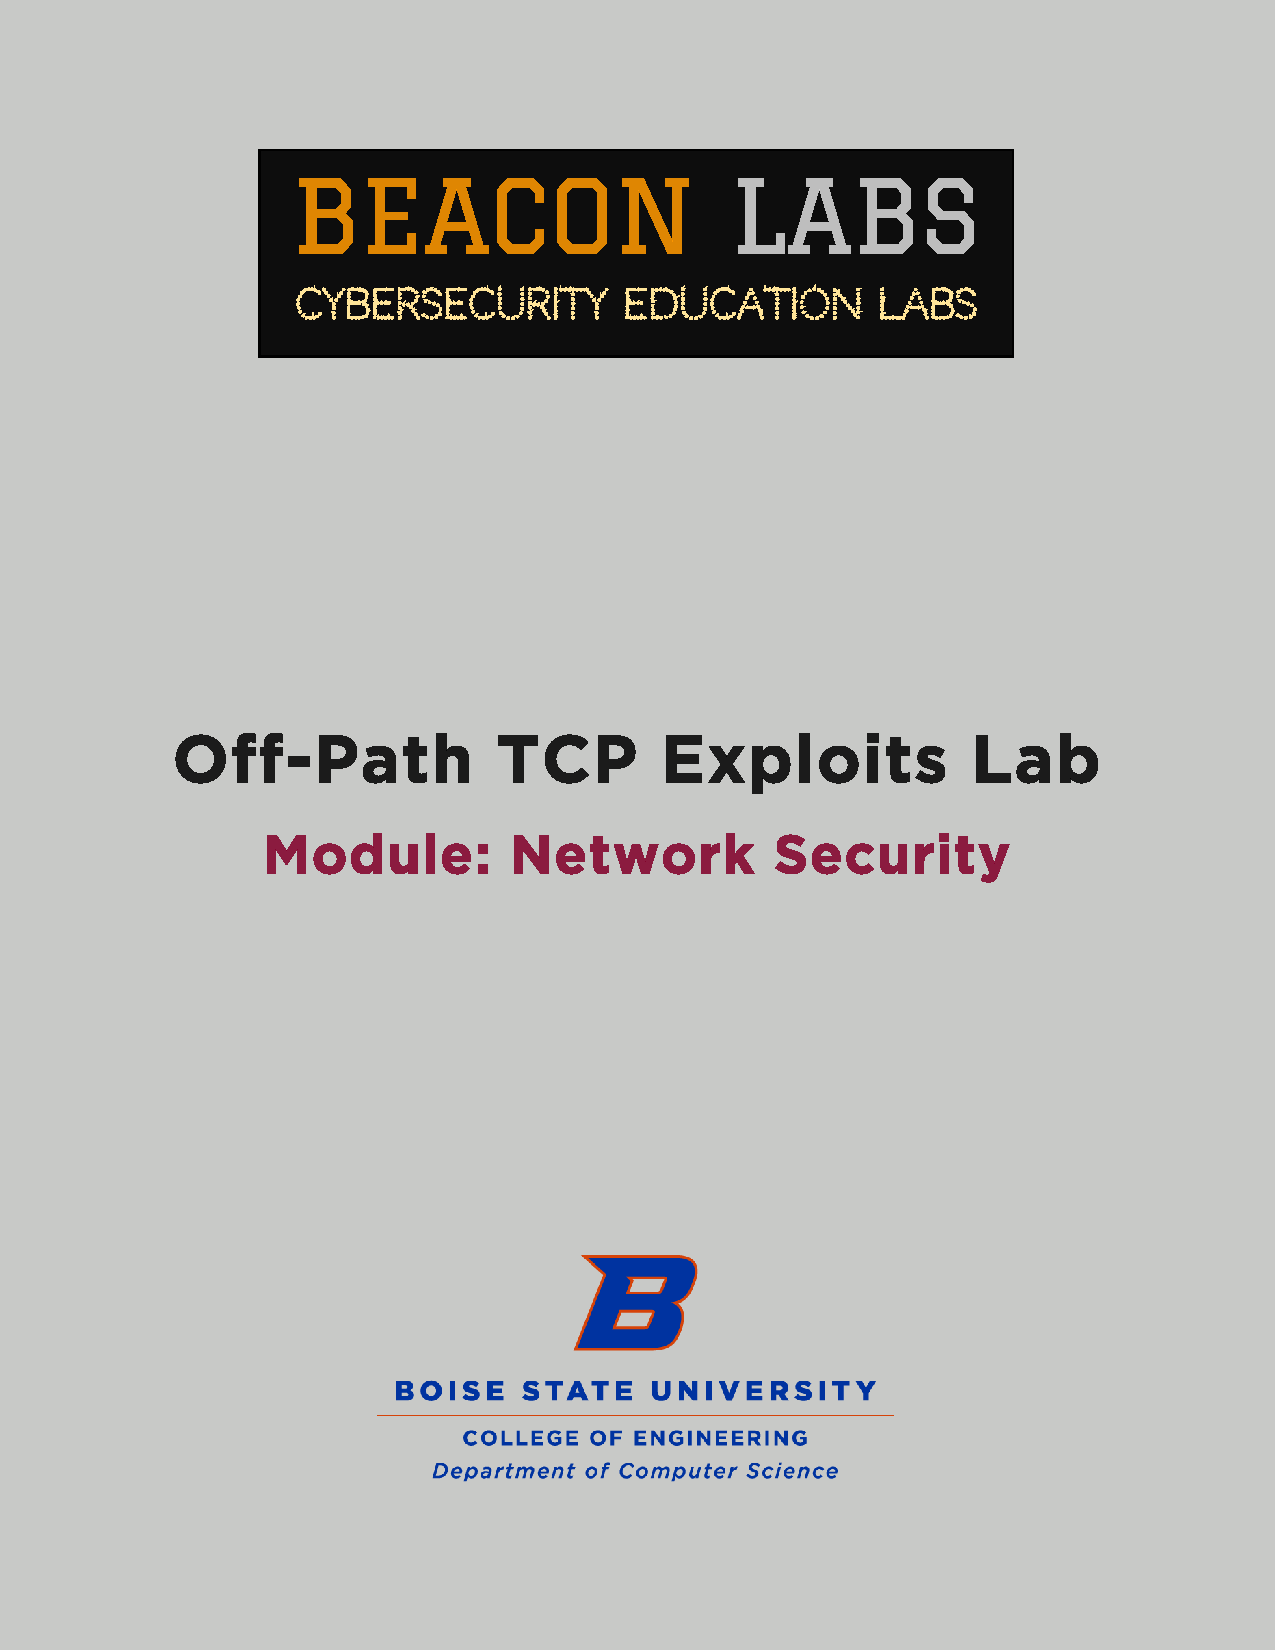
\includepdf[pages=1]{./graphics/1FP.pdf}

\mdfdefinestyle{code}{%
    linecolor=black,
    outerlinewidth=2pt,
    %roundcorner=20pt,
    innertopmargin=4pt,
    innerbottommargin=4pt,
    innerrightmargin=4pt,
    innerleftmargin=4pt,
        leftmargin = 4pt,
        rightmargin = 4pt
    backgroundcolor=black!10
    }

\setcounter{tocdepth}{4}
\setcounter{secnumdepth}{4}

%%%%%%%%%%%%%%%%%%%%%%%%%%%%%%%%%%%%%%%%%
%%% URL style same as regular text
%%%%%%%%%%%%%%%%%%%%%%%%%%%%%%%%%%%%%%%%%
	
\urlstyle{same}

%%%%%%%%%%%%%%%%%%%%%%%%%%%%%%%%%%%%%%%%%
%%% Deliverable Information
%%%%%%%%%%%%%%%%%%%%%%%%%%%%%%%%%%%%%%%%%

% Project Meta Information
\ProjectFullTitle{Beacon Network Security Labs: Off-Path TCP Exploits Lab}
\ProjectAcronym{HYPERRIDE}
\ProjectRefNo{957788}

% Report Number, use either "1", "2", or "3" for the corresponding reporting period
\delivNumber{0}

% Period covered by the report
\delivFrom{dd/mm/yyyy}
\delivTo{dd/mm/yyyy}

% Report Responsible Partner
\delivResponsible{AIT Austrian Institute of Technology (AIT)} 

% Report Version, Contractual and Actual Date, Dissemination Level, Type
\delivVersion{vn.n}
\ContractualDate{dd/mm/yyyy}
\ActualDate{dd/mm/yyyy}

% List of Main Authors (usually from the responsible partner)
\delivAuthor{[Jordan Whyte, Gaby Dagher]}

% List of Co-Authors (all other co-authors should be listed here)
\delivFPAuthor{[]}

% Report Status
\delivStatus{d} %% d = draft, f = final, s = submitted

%%%%%%%%%%%%%%%%%%%%%%%%%%%%%%%%%%%%%%%%%
%%% Change Log
%%%%%%%%%%%%%%%%%%%%%%%%%%%%%%%%%%%%%%%%%

\istChange{dd/mm/yyyy}{v1.0}{Name (Partner short name)}{Draft report template}
\istChange{}{}{}{}

%%%%%%%%%%%%%%%%%%%%%%%%%%%%%%%%%%%%%%%%%
%%% Cover Page
%%%%%%%%%%%%%%%%%%%%%%%%%%%%%%%%%%%%%%%%%

%\makecover

%%%%%%%%%%%%%%%%%%%%%%%%%%%%%%%%%%%%%%%%%
%%% Table of Contents
%%%%%%%%%%%%%%%%%%%%%%%%%%%%%%%%%%%%%%%%%

\clearpage
\fancypagestyle{plain}{}
\settableofcontents
\tableofcontents
\clearpage

%%%%%%%%%%%%%%%%%%%%%%%%%%%%%%%%%%%%%%%%%
%%% Terminology
%%%%%%%%%%%%%%%%%%%%%%%%%%%%%%%%%%%%%%%%%

\newpage
\section*{\Large {Terminology}}

\begin{description}
\item[\textbf{ ACK-window}] \begin{sloppypar}The ACK-window, or Acknowledgement window, is a concept in TCP (Transmission Control Protocol) that represents the range of acceptable sequence numbers that are acknowledged by the receiving end of a TCP connection.\end{sloppypar}

\item[\textbf{ Blind In-Window Attacks}] \begin{sloppypar}Blind in-window attacks are TCP attacks in which the attacker isn't in the path of data transfer but is able to pose as one side of the TCP exchange by sending packets externally that are "in-window" of the expected packets.\end{sloppypar}

\item[\textbf{ Challenge-ACK}] \begin{sloppypar}Challenge Acknowledgement (Challenge-ACK) is a security feature in the TCP protocol that aims to protect against blind in-window attacks.\end{sloppypar}

\item[\textbf{ Global Rate Limit}] \begin{sloppypar}A mechanism to prevent resource exhaustion attacks by putting a limit on the number of responses (i.e., ACKs) that a server can send.\end{sloppypar}

\item[\textbf{ Acknowledgement Number Inference}] \begin{sloppypar}A technique that is used in network security, particularly in TCP/IP hacking. It entails inferring the sequence of numbers that the receiving end of a TCP connection is expecting next (the ACK numbers) based on observing the pattern of previous ACK numbers.\end{sloppypar}
\end{description}
\normalsize

%%%%%%%%%%%%%%%%%%%%%%%%%%%%%%%%%%%%%%%%%
%%% Overview
%%%%%%%%%%%%%%%%%%%%%%%%%%%%%%%%%%%%%%%%%
\newpage
\section*{Overview}\label{sec:work-carried-out}
\addcontentsline{toc}{section}{Overview}

\textbf{Objective}

Understand the flow of an off-path TCP exploit and gain the ability to execute an off-path TCP exploit through completing the essential code to exploit the Global Rate Limit vulnerability.

\textbf{Off-Path TCP Exploits}

Off-Path TCP Exploits refer to a class of cybersecurity attacks where an attacker can manipulate or infer data from a TCP session between two other parties without being in the data transmission path.

In Linux Kernel version 3.6, RFC (Request For Comment) 5961 was faithfully implemented to stop blind in-window attacks but, it also created a new vulnerability. This vulnerability lies in the Global Rate Limit, which limits the number of challenge-ACKs to 100 per second to prevent excessive resource usage. Figure~\ref{fig:ACK_Window_Illustration} demonstrates this below. 

\begin{figure}[!h]
    \centering
    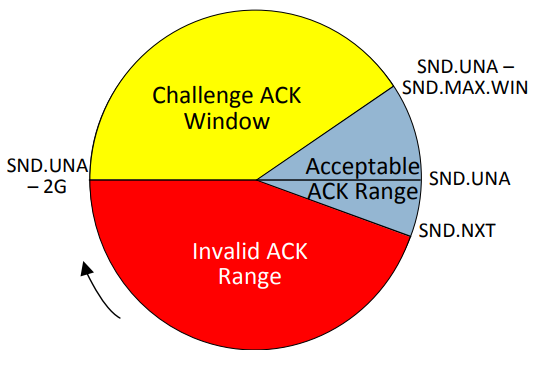
\includegraphics[width=0.6\columnwidth]{ACK_window.png}
    \caption{ACK Window Illustration}
    \label{fig:ACK_Window_Illustration}
\end{figure}

The Global Rate Limit can be exploited to show if a TCP connection is present and, if a TCP connection is found, the Global Rate Limit can then subsequently be used to infer the four-tuple of the client and server, the next acceptable sequence number, and the acknowledgment number. After inference of these three components is completed, it is trivial for an attacker to inject spoofed packets.
\begin{sloppypar}

\end{sloppypar}

\begin{sloppypar}
    
\textbf{Resources}

\textit{Video explaining how the attack works:}

\url{https://www.usenix.org/conference/usenixsecurity16/technical-sessions/presentation/cao}

\textit{Paper that the attack is based upon:}

\url{https://www.cs.ucr.edu/~zhiyunq/pub/sec16_TCP_pure_offpath.pdf} $^\text{[\citeauthor{Cao:2016}]}$


%%%%%%%%%%%%%%%%%%%%%%%%%%%%%%%%%%%%%%%%%
%%% Virtual Machine Setup
%%%%%%%%%%%%%%%%%%%%%%%%%%%%%%%%%%%%%%%%%

\section*{Virtual Machine Setup}\label{sec:Virtual-Machine-Setup}
\addcontentsline{toc}{section}{Virtual Machine Setup}

In this lab, three virtual machines will be needed: the client, server, and attacker. There are only two virtual machine images that need to be downloaded since the client and attacker use the same image. The vitual machines will be referred to as the "Client VM," "Server VM," and "Attacker VM."

A Python script is used to create a simple messaging service between the client and server, thereby creating the TCP connection that will eventually be hijacked. 

The server is running a version of Ubuntu 14.04 that has not been updated. The security updates for this operating system serve to patch the vulnerability being exploited, so it's crucial to avoid any updates. Both the client and attacker are running Ubuntu 16.04 with the libtins libraries installed. These libraries are used to spoof and send packets, so they are necessary to have on the virtual machine for the attacker to utilize.

By interacting with the server as seen in Figure~\ref{fig:Exploiting_Server} on page~\pageref{fig:Exploiting_Server}, all steps of the attack can be completed. After this is completed, it then becomes possible to inject packets imitating the server to the client, as seen Figure~\ref{fig:Imitating_the_Server} on page~\pageref{fig:Imitating_the_Server}.

\begin{figure}[h]
    \centering
    
    \begin{minipage}{0.49\textwidth}
        \centering
        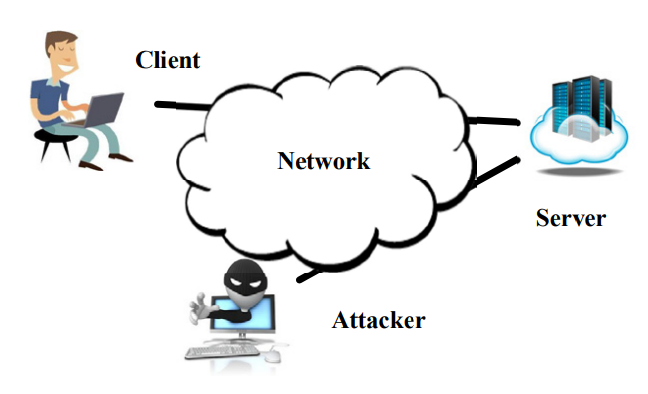
\includegraphics[width=1\textwidth]{Figure_2.png}
        \caption{Exploiting Server}
        \label{fig:Exploiting_Server}
    \end{minipage}
    \hfill
    \begin{minipage}{0.49\textwidth}
        \centering
        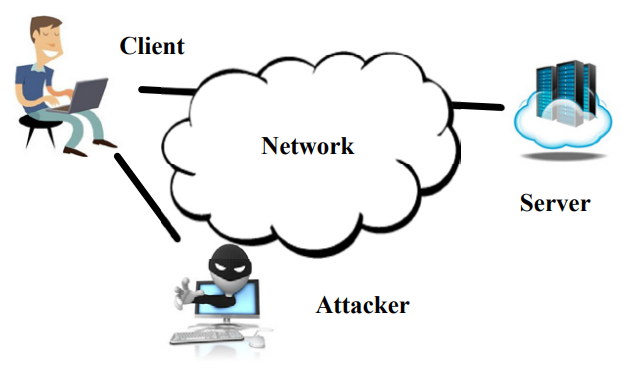
\includegraphics[width=1\textwidth]{Figure_3.png}
        \caption{Imitating the Server}
        \label{fig:Imitating_the_Server}
    \end{minipage}
\end{figure}

For setup instructions, see the provided Setup document.

%%%%%%%%%%%%%%%%%%%%%%%%%%%%%%%%%%%%%%%%%
%%% Lab Task Set 1: Clock Synchronization
%%%%%%%%%%%%%%%%%%%%%%%%%%%%%%%%%%%%%%%%%

\section*{Task Set 1: Clock Synchronization}\label{sec:Task-Set-1}
\addcontentsline{toc}{section}{Task Set 1: Clock Synchronization}

When working with the clock throughout this lab, it's imperative that we tell the program to wait until the clock hits a certain time rather than telling it to sleep for a certain period of time. Keep this in mind while completing the lab.

\textbf{Objective}

Synchronize the Attacker VM's clock with the server clock on the Server VM such that all the packets sent from the Attacker arrive within the proper time interval.

\subsection*{Task 1.1: Initiate a Legitimate TCP Connection}\label{sec:Task-1.1-Initiate-a-Legitimate-TCP-Connection}
\addcontentsline{toc}{subsection}{Task 1.1: Initiate a Legitimate TCP Connection}

A legitimate TCP connection first needs to be established by sending the appropriate flags to the server.

Begin by going to the Attacker VM and opening a terminal. Navigate to the "{\raise.17ex\hbox{$\scriptstyle\mathtt{\sim}$}}/Documents/attacker\_cpp" directory and then open the C++ file that needs to be edited with the following command:

\bigskip

\begin{mdframed}[backgroundcolor=black!10,style=code,nobreak=true,align=center,userdefinedwidth=14cm]
\$ gedit synchronize\_clock.cpp
\end{mdframed}
\bigskip

\colorbox{lightblue}{%
\parbox{\dimexpr\linewidth-2\fboxsep}{%
\textbf{Action}

1.1.1 - Choose the correct TCP flags to initiate the TCP connection.\\
1.1.2 - Write the flag to initialize the TCP connection on line 25 of synchronize\_clock.cpp.\\
1.1.3 - On line 47, disable the flag you set on line 25.\\
1.1.4 - On line 48, set the flag that indicates that the response from the server has been received.\\
(Figure~\ref{fig:synchronize_clock.cpp}, page~\pageref{fig:synchronize_clock.cpp}). 
   }%
}%

\bigskip
\begin{figure}[!h]
    \centering
    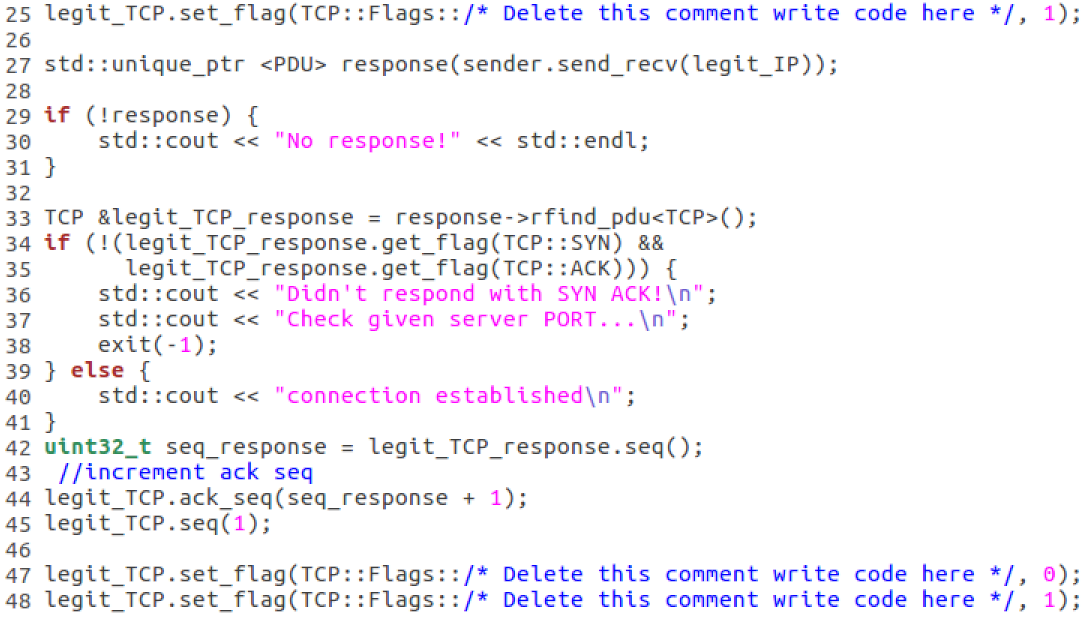
\includegraphics[width=1\columnwidth]{graphics/synchronize_clock Step 1_re.png}
    \caption{synchronize\_clock.cpp Step 1}
    \label{fig:synchronize_clock.cpp}
\end{figure}

\bigskip
\bigskip
\subsection*{Task 1.2: Send 200 Packets Equally Spaced}\label{sec:Task-1.2-Send-200-Packets-Equally-Spaced}
\addcontentsline{toc}{subsection}{Task 1.2: Send 200 Packets Equally Spaced}

The next step in synchronizing the clock is to send 200 packets that are equally spaced in the span of one second to see how many challenge-acks this prompts. Since only 100 challenges can be sent within a second, it can be concluded that the clock is synchronized when only 100 challenges are received.

There is a chance that the clock will already be synchronized, but it is far more likely that more than 100 challenges will be received. This process is attempted twice, adjusting the time between the first and second attempts. The third attempt uses the calculated time delay necessary to receive only 100 challenges.

\colorbox{lightblue}{%
\parbox{\dimexpr\linewidth-2\fboxsep}{%
\textbf{Action}

1.2.1 - Write the necessary line of code to equally space out the 200 packets in the span of one second so that each packet has an equal amount of time between the previous and next packets on line 75 of synchronize\_clock.cpp for round one as seen in Figure~\ref{fig:synchronize_clock2.cpp} below.\\
    }%
}%

\begin{figure}[!h]
    \centering
    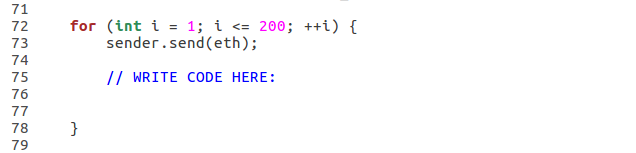
\includegraphics[width=1.1\columnwidth]{graphics/synchronize_clock Step 2.png}
    \caption{synchronize\_clock.cpp Step 2}
    \label{fig:synchronize_clock2.cpp}
\end{figure}

\subsection*{Task 1.3: Adjust Time Delay}\label{sec:Task-1.3-Adjust-Time-Delay}
\addcontentsline{toc}{subsection}{Task 1.3: Adjust Time Delay}

Prior to beginning round two, we need to shift the time that we start sending packets by 5 milliseconds. After the 5 milliseconds is up, we must perform the same process of sending out 200 equally spaced packets in the span of one second and then checking the number of challenges we received back. Just like in round 1, if we received 100 challenges then our clock is now synchronized and if we received more than 100 challenges, we need to continue on with round 3.

\colorbox{lightblue}{%
\parbox{\dimexpr\linewidth-2\fboxsep}{%
\textbf{Action}

1.3.1 - Write your code on line 98 for round two as seen in Figure~\ref{fig:synchronize_clock3.cpp} on page~\pageref{fig:synchronize_clock3.cpp} below.
    }%
}%

\begin{figure}[!h]
    \centering
    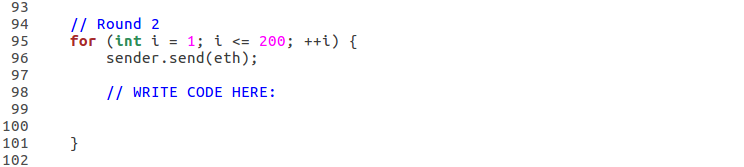
\includegraphics[width=1.2\columnwidth]{graphics/synchronize_clock Step 3.png}
    \caption{synchronize\_clock.cpp Step 3}
    \label{fig:synchronize_clock3.cpp}
\end{figure}

\subsection*{Task 1.4: Add the variable of n\_result}
\addcontentsline{toc}{subsection}{Add The Variable of n\_result}

If round 3 has been reached, that means that we have more information to work with. Specifically, we can compare the number of packets received in round 1 to the number of packets received in round 2.

Let's assume that in round 1, $x$ RST packets were sent to the server over the first second and in the second second, $y$ RST packets were sent to the server. Note that $x + y = 200$. In round 2, we can assume that $(x - 1)$ RST packets were sent to the server in the first second and $(y + 1)$ RST packets were sent to the server in the second second due to the attacker waiting those 5 milliseconds before starting round 2. Therefore, we can calculate the number of packets from round 1 and round 2 as:

$$ n_1 = min(x, 100) + min(y, 100) $$
$$ n_2 = min(x - 1, 100) + min(y + 1, 100) $$

Therefore, if $n_2 \geq n_1$ then we can assume that $y \geq 100$ and $x \leq 100$ which means that  $n_1 = x + 100$ and $n_2 = (x-1) + 100 < n_1$ which contradicts $n_2 \geq n_1$. Therefore, $y < 100$ and $x > 100$ which means that $n_2 = 100 + (y + 1) = 100 + (200 - x + 1)$ which can be simplified to: $(x-1) = 300 - n_2$. From this, the attacker will know that in the event that $n_2 >= n_1$, they will need to wait $(300-n_2)\cdot\frac{1}{200}$ seconds to synchronize their clock with the server's clock.

Likewise, if $n_1 > n_2$ then the attacker will know that $y > 100$ and $x < 100$ which means that $n_2 = (x - 1) + 100$ and therefore the attacker will need to wait $\frac{n_2 - 100}{200}$ seconds to synchronize their clock with the server's clock.

\textit{Note:} in the code you'll see the calculation is slightly different. This is because the conversion from seconds to milliseconds has been done and simplified. I.e., $\frac{n_2 - 100}{200} \cdot 1000 = (n_2 - 100) * 5 $

\colorbox{lightblue}{%
\parbox{\dimexpr\linewidth-2\fboxsep}{%
\textbf{Action}

1.4.1 - Write your code on line 127 for round three as seen in Figure~\ref{fig:synchronize_clock4.cpp} below.
    }%
}%

\begin{figure}[!h]
    \centering
    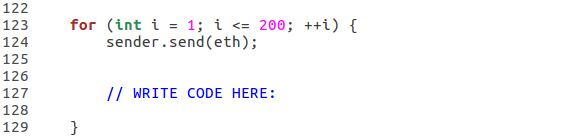
\includegraphics[width=1\columnwidth]{graphics/synchronize_clock Step 4.png}
    \caption{synchronize\_clock.cpp Step 4}
    \label{fig:synchronize_clock4.cpp}
\end{figure}

After altering and saving the code, compile it by running the following command:

\bigskip

\begin{mdframed}[backgroundcolor=black!10,style=code,nobreak=true,align=center,userdefinedwidth=14cm]
    \$ rm -f exploit \&\& make
\end{mdframed}

\bigskip

You can then run the partial exploit by executing the following command:

\bigskip

\begin{mdframed}[backgroundcolor=black!10,style=code,nobreak=true,align=center,userdefinedwidth=14cm]
    \$ sudo ./exploit <client\_ip> <server\_ip> <server\_port>
\end{mdframed}

\bigskip

If all tasks in this task set are done properly, you should see "CLOCK SYNCHRONIZATION COMPLETE" appear as output in the terminal.

There is a redundancy in the code to try the time synchronization again in case there was any packet loss. If the code is written correctly by the student it should only take one round to complete but there is a possibility it will need a second or third.

%%%%%%%%%%%%%%%%%%%%%%%%%%%%%%%%%%%%%%%%%
%%% Lab Task Set 2: Four-Tuple Inference
%%%%%%%%%%%%%%%%%%%%%%%%%%%%%%%%%%%%%%%%%

\section*{Task Set 2: Four-Tuple Inference}\label{sec:Task-Set-2}
\addcontentsline{toc}{section}{Task Set 2: Four-Tuple Inference}

\textbf{Objective}

Infer the four-tuple of the client and server to then utilize the four-tuple in the identification of the correct client port.

\bigskip

This task set will be conducted in the 4tuple\_inference.cpp file.

Use the following command to open the correct file:

\bigskip

\begin{mdframed}[backgroundcolor=black!10,style=code,nobreak=true,align=center,userdefinedwidth=14cm]
    \$ gedit 4tuple\_inference.cpp
\end{mdframed}

\subsection*{Task 2.1: Send SYN-ACK Packets}\label{sec:Task-2.1-Send-SYN-ACK-Packets}
\addcontentsline{toc}{subsection}{Task 2.1: Send SYN-ACK Packets}

Over the course of a second, SYN-ACK packets are sent out to the server with the four-tuples of <srcIP = clientIP, dstIP = serverIP, srcPort = X, dstPort = serverPort>. The source port is labeled as X as it is the part that needs to be figured out. The default Linux port range is 32768 to 61000. By halving this and sending packets to ports in the range 46884 - 61000, it's possible to determine which part of this range contains the correct port number.

Once SYN-ACK packets have been sent out in the first half, 100 RST packets can be sent in the same second. If 100 challenge-ACKs are observed, it can be inferred that it's in the first half of the search space. If 99 are observed, it can be inferred that one was sent to the client, and thus the correct port is in the second half. The observed amount is used to determine if the correct client port is within the searched range and how the right or left port should be adjusted accordingly.

\colorbox{lightblue}{%
\parbox{\dimexpr\linewidth-2\fboxsep}{%
\textbf{Action}

2.1.1 - In `4tuple\_inference.h', update the port constants to accurately \\ reflect the default Linux port range. \\
2.1.2 - Remove lines 12-16 and lines 119-128, inclusive. \\
2.1.3 - Complete the binary search algorithm by writing your code on \\ line 67 as seen in Figure~\ref{fig:4tuple_inference.cpp} on page~\pageref{fig:4tuple_inference.cpp} below.
    }%
}%

\begin{figure}[!h]
    \centering
    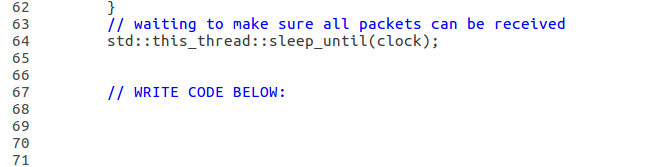
\includegraphics[width=1.1\columnwidth]{graphics/4tuple_inference Step 1.png}
    \caption{4tuple\_inference.cpp Step 1}
    \label{fig:4tuple_inference.cpp}
\end{figure}

After altering and saving the code, compile it by following the same steps as described previously. If the code is written correctly, the terminal should read "Client port:\#\#\#\#\#" where "\#\#\#\#\#" is the same as the "client port" shown in the Server VM's terminal. After finding the client port, the next step is to locate the sequence number.

%%%%%%%%%%%%%%%%%%%%%%%%%%%%%%%%%%%%%%%%%
%%% Lab Task Set 3: Sequence Number Inference
%%%%%%%%%%%%%%%%%%%%%%%%%%%%%%%%%%%%%%%%%

\section*{Task Set 3: Sequence Number Inference \& Nash Equilibrium}\label{sec:Task-Set-3}
\addcontentsline{toc}{section}{Task Set 3: Sequence Number Inference \& Nash Equilibrium}

\textbf{Objective}

Infer the sequence number such that the Attacker's packets are received in the desired order.

\bigskip

This task set will be conducted in the sequence\_inference.cpp file. Use the following command to open the correct file:

\bigskip

\begin{mdframed}[backgroundcolor=black!10,style=code,nobreak=true,align=center,userdefinedwidth=14cm]
\$ gedit sequence\_inference.cpp
\end{mdframed}

\bigskip

\subsection*{Task 3.1: Determine the Correct Sequence Number}\label{sec:Task-3.1-Determine-the-Correct-Sequence-Number}
\addcontentsline{toc}{subsection}{Task 3.1: Determine the Correct Sequence Number}

First, it is necessary to determine the correct sequence number. This is done by sending packets to each block of the sequence number space and observing the server's response.

\colorbox{lightblue}{%
\parbox{\dimexpr\linewidth-2\fboxsep}{%
\textbf{Action}

3.1.1 - Remove lines 21-26, 55-59, 62, 63, and 67 inclusive.\\
3.1.2 - Analyze the game theory table provided below in Table~\ref{Tab:game_theory} on page~\pageref{Tab:game_theory} and decide whether to search high or low first.\\
3.1.3 - Explain your decision in your lab report.\\
3.1.4 - Complete the for-loop conditions (initialization, condition, and increment/decrement) on line 61 of `sequence\_inference.cpp' to reflect your decision.\\
    }%
}%

\begin{table}[ht]
    \setlength{\extrarowheight}{2pt}
    \begin{tabular}{cc|c|c|}
        & \multicolumn{1}{c}{} & \multicolumn{2}{c}{\color{blue}Defender}\\
        & \multicolumn{1}{c}{} & \multicolumn{1}{c}{\color{blue}Start Low}  & \multicolumn{1}{c}{\color{blue}Start High} \\\cline{3-4}
        \color{red}\multirow{2}*{Attacker}  & \color{red}Search Low & $\color{red}(2,\color{blue}-2)$ & $\color{red}(2,\color{blue}-2)$ \\\cline{3-4}
        & \color{red}Search High & $\color{red}(1,\color{blue}-1)$ & $\color{red}(3,\color{blue}-3)$ \\\cline{3-4}
    \end{tabular}
    \caption{Game theory table representing the advantages and disadvantages of both (the attacker and the defender)}
    \label{Tab:game_theory}
\end{table}

The defender has the option of starting the sequence number with a high value or a low value. Starting with a high value costs more resources, so it gives the attacker $2$ and the defender $-2$. If the defender starts it at a low value, then it's $1$ and $-1$ instead. If the attacker chooses correctly to search high or low first, then another $1$ and $-1$ are given to the attacker and defender, respectively.

\subsection*{Task 3.2: Narrowing Down the Search Space}\label{sec:Task-3.2-Narrowing-Down-the-Search-Space}
\addcontentsline{toc}{subsection}{Task 3.2: Narrowing Down the Search Space}

The next step in the exploit is to narrow the search space down to a single block. This is done through another binary search in which we observe how many packets are received after sending them to one half of the search space at a time.

The definitions of the variables are as follows:

\bigskip

\begin{description}
    \item[\textbf{SEQ\_MAX}] \begin{sloppypar}is the maximum value a 32-bit integer can be.\end{sloppypar}

    \item[\textbf{WINDOW\_SIZE}] \begin{sloppypar}is 12,600 as that is the default window size for Linux.\end{sloppypar}

    \item[\textbf{chunk\_size}] \begin{sloppypar}is 8,000 which is the area where a packet is sent to each round.\end{sloppypar}

    \item[\textbf{SEQ\_MAX/chunk\_size/WINDOW\_SIZE}] \begin{sloppypar} is the maximum chunk\_id to be searched.\end{sloppypar}
\end{description}

\subsection*{Task 3.3: Find the Sequence Number}\label{sec:Task-3.3-Find-the-Sequence-Number}
\addcontentsline{toc}{subsection}{Task 3.3: Find the Sequence Number}

We can find the correct sequence number through a three step process:

\begin{enumerate}
    \item Approximate the range in which the number lies.
    \item Find the correct block.
    \item Find the sequence number itself.
\end{enumerate}

The search space is narrowed down to a single block through another binary search algorithm, similarly to the 4-tuple inference. The search space is then progressively narrowed down by observing the number of packets received after sending packets to one half of the space. You will \textbf{not} have to write any code for this step.

The iteration through sequence numbers will continue until the correct sequence number is found. Once the correct sequence number is found, we'll infer the next acknowledgement number. You will \textbf{not} have to write any code for this step either.

Complete the final step of this task by doing the following:

\colorbox{lightblue}{%
\parbox{\dimexpr\linewidth-2\fboxsep}{%
\textbf{Action}

3.3.1 - Write the code to send packets on the legitimate connection to exhaust the global rate limit on line 73 of `sequence\_inference.cpp'.\\
3.3.2 - Create an if-statement to check if the correct block is in the current search space on line 91 of sequence\_inference.cpp as seen in Figure~\ref{fig:sequence_inference} on page~\pageref{fig:sequence_inference} below.
    }%
}%

\begin{figure}[!h]
    \centering
    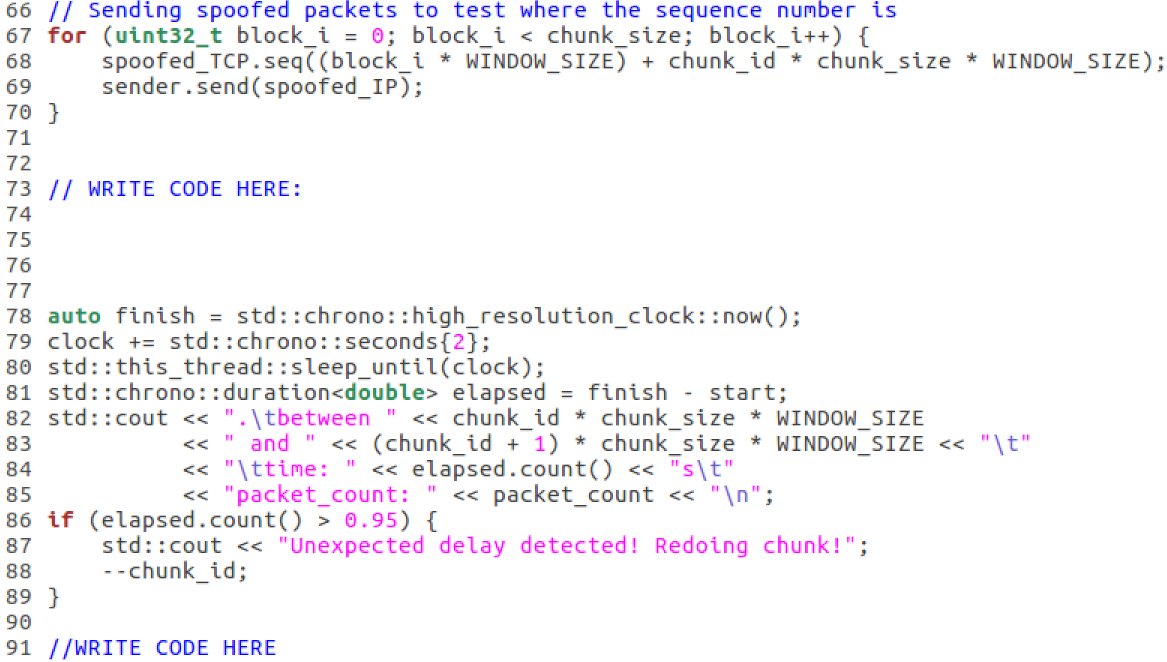
\includegraphics[width=1\columnwidth]{graphics/sequence_inference Step 1.png}
    \caption{sequence\_inference.cpp Step 1}
    \label{fig:sequence_inference}
\end{figure}

After altering and saving the code, compile it using the same process as before.

%%%%%%%%%%%%%%%%%%%%%%%%%%%%%%%%%%%%%%%%%
%%% Lab Task Set 4: Acknowledgement Number Inference
%%%%%%%%%%%%%%%%%%%%%%%%%%%%%%%%%%%%%%%%%

\section*{Task Set 4: Acknowledgement Number  Inference}\label{sec:Task-Set-4}
\addcontentsline{toc}{section}{Task Set 4: Acknowledgement Number Inference}

\textbf{Objective}

Infer the next expected acknowledgement number from the server such that the Attacker's packets are acknowledged in the proper order.

\bigskip

This task set will be conducted in the ack\_inference.cpp file. Use the following command to open the correct file:

\bigskip

\begin{mdframed}[backgroundcolor=black!10,style=code,nobreak=true,align=center,userdefinedwidth=14cm]
    \$ gedit ack\_inference.cpp
\end{mdframed}

\bigskip

\subsection*{Task 4.1: Determine the Correct Acknowledgement Number}\label{sec:Task-3.1-Determine-the-Correct-Acknowledgement-Number}
\addcontentsline{toc}{subsection}{Task 4.1: Determine the Correct Acknowledgement Number}

To find the next expected acknowledgement number of the server, a multi-bin search is used. The maximum window size for acknowledgement numbers is $2^{30}$. This is defined in the code as $one\_G$. By sending one packet to the $0$ sequence number, two to $one\_G - 1$, four to $two\_G - 1$, and eight to $three\_G - 1$, the amount of packets received can be counted to find the area in which the correct number lies. For instance, if 94 challenges are received, then it indicates that challenges from $one\_G$ and $two\_G$ have been triggered, thus the range is in between the two of them. If 96 challenges are observed, then it indicates that challenges from only $two\_G$ have been triggered, thus the range is inside of $two\_G$.

\colorbox{lightblue}{%
\parbox{\dimexpr\linewidth-2\fboxsep}{%
\textbf{Action}

4.1.1 - Write code to handle missing four packets on line 89, eight packets on line 100, and 12 packets on line 111 of ack\_inference.cpp as seen in Figure~\ref{fig:ack_inference} below.
    }%
}%

\begin{figure}[!h]
    \centering
    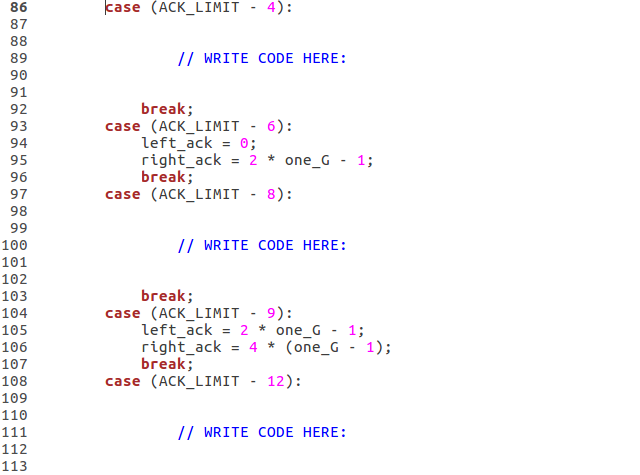
\includegraphics[width=1\columnwidth]{graphics/ack_inference.png}
    \caption{ack\_inference.cpp}
    \label{fig:ack_inference}
\end{figure}

\bigskip

After altering the code, compile it by navigating to the attacker\_cpp folder through the terminal, removing the exploit.exe file, and then entering the make command.

Once this is completed the left boundary of the acceptable ACK range can be found and spoofed packets can be sent to the client.

If all the code is working correctly, you should be able to write messages into the console that will show up as the server in the client’s messaging terminal.

%%%%%%%%%%%%%%%%%%%%%%%%%%%%%%%%%%%%%%%%%
%%% Submission
%%%%%%%%%%%%%%%%%%%%%%%%%%%%%%%%%%%%%%%%%

\section*{Submission}\label{sec:Submission}
\addcontentsline{toc}{section}{Submission}

Submit a lab report using the provided \href{https://docs.google.com/document/d/1f_rB22EzL8aezExZ7jYFARnuy5xuhcwC/edit?usp=sharing&ouid=113481593569562690929&rtpof=true&sd=true}{lab report template}. Create a lab report that consists of text and images from each task in the lab. Describe the process you went through to solve each task. Be sure to include how you solved the game theory table. With your submission include the synchronize\_clock.cpp, 4tuple\_inference.cpp, sequence\_inference.cpp, and ack\_inference.cpp files.
\end{sloppypar}

\section*{Summary}\label{sec:Summary}
\addcontentsline{toc}{section}{Summary}

In this lab you've learned what an Off-Path TCP attack is, how it's implemented, and what an attacker can do with it.

Off-Path TCP attacks are of particular concern for public networks since the networks are inherently less secure. As a consequence of this, Off-Path TCP attacks are far easier for an attacker to perform on public networks so, knowing how this attack works and is performed will be beneficial for determining appropriate defensive measures.

\bibliography{References}
\bibliographystyle{plain}

\end{document}

%%%%%%%%%%%%%%%%%%%%%%%%%%%%%%%%%%%%%%%%%